\documentclass[column,amsmath,amssymb,floatfix]{revtex4}

% ---- Pacotes matemáticos essenciais ----
\usepackage{amsmath}
\usepackage{amssymb}
\usepackage{amsfonts}

% ---- Pacotes para gráficos e figuras ----
\usepackage{graphicx}
\usepackage{subcaption}
\usepackage{float}

% ---- Pacotes para formatação ----
\usepackage{xcolor}
\usepackage{bm}
\usepackage{titlesec}
\usepackage{enumitem}

% ---- Bibliografia ----
\usepackage[style=apa]{biblatex}
\addbibresource{referencias.bib}

% ---- Código fonte ----
\usepackage{listings}

\lstdefinestyle{customc}{
  belowcaptionskip=1\baselineskip,
  breaklines=true,
  frame=none,
  xleftmargin=\parindent,
  language=python,
  showstringspaces=false,
  basicstyle=\footnotesize\ttfamily,
  keywordstyle=\bfseries\color{green!40!black},
  commentstyle=\itshape\color{purple!40!black},
  identifierstyle=\color{blue},
  stringstyle=\color{orange},
}

\lstset{
 escapechar=@,
 style=customc,
 inputencoding=utf8, 
 extendedchars=true,
 literate={á}{{\'{a}}}1 {ã}{{\~{a}}}1 {é}{{\'{e}}}1 {ê}{{\^{e}}}1 {í}{{\'{i}}}1 
          {ó}{{\'{o}}}1 {õ}{{\~{o}}}1 {ú}{{\'{u}}}1 {ç}{{\c{c}}}1,
 keepspaces=true,
 columns=flexible,
 basicstyle=\ttfamily
}

% ---- Idioma e codificação ----
\usepackage[brazilian]{babel}
\usepackage[utf8]{inputenc}
\usepackage[T1]{fontenc}

% ---- Hiperlinks ----
\usepackage{hyperref}

% ---- Comandos personalizados ----
\newcommand{\PAR}[1]{\left({[#1]}\right)}

% ---- Ajustes de espaçamento para títulos ----
\titlespacing\section{0pt}{12pt plus 4pt minus 2pt}{8pt plus 2pt minus 2pt}
\titlespacing\subsection{0pt}{12pt plus 4pt minus 2pt}{8pt plus 2pt minus 2pt}
\titlespacing\subsubsection{0pt}{12pt plus 4pt minus 2pt}{0pt plus 2pt minus 2pt}

\begin{document}

\title{Estudo do Método de Diferenças Finitas para Equação da Onda unidimencional}

\author{Lucas Amaral Taylor}

\begin{center}
	\begin{abstract}
		\baselineskip 11pt
		Neste trabalho, aplicaremos o Método de Diferenças Finitas (MDF) para resolução numérica de equações de onda unidimensional em três exemplos pré-selecionados no enunciado.
	\end{abstract}
\end{center}


\maketitle

\section{Introdução} 
No enunciado do trabalho foram passados três exemplos, exercícios-problema, em cada um deles, vamos desenvolver o que está sendo solicitado. De maneira, geral, os três exemplos, seguem como estrutura a plotagem de dados e o cálculo do erro. Para essas duas tarefas, utilizaremos o Método de Diferenças Finitas (MDF) aplicado junto à linguagem de \texttt{Python} com auxílo das bibliotecas \texttt{numpy} e \texttt{matplotlib.pyplot}.

\section{Descrição da parte teórica do trabalho}
No presente relatório, aplicaremos o Método de Diferenças Finitas (MDF) para resolução da \textit{equação da velocidade da onda} dada por:
\begin{equation}
	u_{tt} = c^2 u_{xx}, \quad c>0.
	\label{eq:equacao-da-onda}
\end{equation}
em três problemas distintos. Em cada um deles, são fornecidas condições iniciais:
\begin{equation}
	u(x,0) = \Phi(x) \quad \text{ e } \quad u_t(x, 0) = \Psi(x)
	\label{eq:condicao-inicial-onda}
\end{equation}

Para a resolução, utilizaremos o esquema de diferenças finitas dado por:
\begin{align}
	U_m^{n+1} & = c^2\lambda^2(U_{m-1}^n + U_{m+1}^n) + 2(1-c^2\lambda^2)U_m^n - U_m^{n-1} \label{eq:edf-principal}                  \\
	U_m^0     & = \Phi(x_m) \label{eq:edf-inicial}                                                                                   \\
	U_m^1     & = \frac{c^2\lambda^2}{2}(\Phi_{m-1} + \Phi_{m+1}) + (1-c^2\lambda^2)\Phi_m + \tau\Psi_m \label{eq:edf-passo-inicial} 
\end{align}

As condições de fronteira consideradas são:
\begin{enumerate}[label=\roman*.]
	\item Dirichlet: $u(a,t) = \alpha(t)$ ou $u(b,t) = \beta(t)$
	\item Neumann: $u_x(a,t) = \phi(t)$ ou $u_x(b,t) = \psi(t)$
	\item Combinação das anteriores
\end{enumerate}

Utilizamos as seguintes aproximações para cada condição de fronteira:
\begin{enumerate}[label=\roman*.]
	\item Para Dirichlet:
	      \begin{align}
	      	\text{Se } u(a,t) & = \alpha(t): U_0^{n+1} = \alpha(t_{n+1}) \label{eq:dirichlet-a} \\
	      	\text{Se } u(b,t) & = \beta(t): U_M^{n+1} = \beta(t_{n+1}) \label{eq:dirichlet-b}   
	      \end{align}
	\item Para Neumann de ordem 1:
	      \begin{align}
	      	\text{Se } u_x(a,t) & = \phi(t): U_0^{n+1} = U_1^{n+1} - h\phi(t_{n+1}) \label{eq:neumman-1-a}     \\
	      	\text{Se } u_x(b,t) & = \psi(t): U_M^{n+1} = U_{M-1}^{n+1} + h\psi(t_{n+1}) \label{eq:neumman-1-b} 
	      \end{align}
	      	      	      	      
	\item Para Neumann de ordem 2:
	      \begin{align}
	      	\text{Se } u_x(a,t) & = \phi(t): U_0^{n+1} = \frac{4U_1^{n+1} - U_2^{n+1} - 2h\phi(t_{n+1})}{3}\label{eq:neumman-2-a}         \\
	      	\text{Se } u_x(b,t) & = \psi(t): U_M^{n+1} = \frac{4U_{M-1}^{n+1} - U_{M-2}^{n+1} + 2h\psi(t_{n+1})}{3}\label{eq:neumman-2-b} 
	      \end{align}    
\end{enumerate}

onde:
\begin{itemize}
	\item $u(x,t)$ é a solução exata no ponto $x$ e no instante $t$
	\item $U_m^n$ é a aproximação numérica de $u(x_m,t_n)$
	\item $c$ é a velocidade da onda
	\item $h$ é o espaçamento da malha espacial
	\item $\tau$ é o espaçamento da malha temporal
	\item $\lambda = \tau/h$ é a razão entre os espaçamentos
	\item $M$ é o número de pontos da malha espacial
	\item $x_m = a + mh$ são os pontos da malha espacial
	\item $t_n = n\tau$ são os pontos da malha temporal
	\item $\Phi(x)$ é a condição inicial de posição
	\item $\Psi(x)$ é a condição inicial de velocidade
\end{itemize}

\section{Implementação e explicação da resolução da tarefa}

A respeito da implementação da tarefa, temos que foi utilizado o ambiente \textit{Python} e as bibliotecas \texttt{matplotlib.pyplot} e \texttt{numpy}. Por questão de simplicidade, o programa foi desenvolvido em um único arquivo, \texttt{main.py}. O programa \texttt{main.py} é constituído por uma função principal, a função \texttt{main()} e outras cinco funções.

No que diz respeito à função \texttt{main()}, trata-se de um controle de fluxo para o usuário selecionar o exemplo trabalhado. No que diz respeito às outras, temos duas funções principais: \texttt{resolve\_eq\_onda()} e a função \texttt{aplica\_cond\_contorno()}, e três funções dedicadas a cada exemplo proposto pelo enunciado: \texttt{exemplo01()}, \texttt{exemplo02()} e \texttt{exemplo03()}. No presente relatório, vamos realizar uma análise mais profunda nas duas primeiras funções citadas e pontuar as particularidades das funções dedicadas à cada exemplo.



\subsection{Função \texttt{resolve\_eq\_onda()}}

A função \texttt{resolve\_eq\_onda()} é dada por:

\begin{lstlisting}
def resolve_eq_onda(a, b, T, h, lambda_val, c=1.0, phi=None, psi=None,
                    cont_esq=None, cont_dir=None,
                    tipo_cont_esq='dirichlet',
                    tipo_cont_dir='dirichlet',
                    ordem_neumann=2):
                      
    # Discretização do domínio 
    M = int((b - a) / h)
    tau = lambda_val * h
    N = int(T / tau)

    x = np.linspace(a, b, M + 1)
    t = np.linspace(0, T, N + 1)
    U = np.zeros((N + 1, M + 1))

    # Condições iniciais
    if phi is not None:
        U[0, :] = phi(x)
    if psi is not None:
        # Primeiro passo temporal (ordem 2)
        U[1, 1:-1] = (c ** 2 * lambda_val ** 2 / 2) * (U[0, :-2] + U[0, 2:]) + \
                     (1 - c ** 2 * lambda_val ** 2) * U[0, 1:-1] + \
                     tau * psi(x[1:-1])
        U[1, 0] = aplica_cond_contorno(U, t, 1, 0, cont_esq, tipo_cont_esq, h, ordem_neumann)
        U[1, -1] = aplica_cond_contorno(U, t, 1, M, cont_dir, tipo_cont_dir, h, ordem_neumann)

    # Esquema explícito para demais passos
    for n in range(1, N):
        U[n + 1, 1:-1] = c ** 2 * lambda_val ** 2 * (U[n, :-2] + U[n, 2:]) + \
                         2 * (1 - c ** 2 * lambda_val ** 2) * U[n, 1:-1] - \
                         U[n - 1, 1:-1]
        U[n + 1, 0] = aplica_cond_contorno(U, t, n + 1, 0, cont_esq, tipo_cont_esq, h, ordem_neumann)
        U[n + 1, -1] = aplica_cond_contorno(U, t, n + 1, M, cont_dir, tipo_cont_dir, h, ordem_neumann)

    return U, x, t

\end{lstlisting}
A função \texttt{resolve\_eq\_onda()} recebe os seguintes parâmetros:
\begin{itemize}
	\item \texttt{a, b}: Limites do intervalo espacial $[a,b]$
	\item \texttt{T}: Tempo final da simulação
	\item \texttt{h}: Passo espacial (discretização em $x$)
	\item \texttt{lambda\_val}: Razão $\tau/h$, onde $\tau$ é o passo temporal 
	\item \texttt{c}: Velocidade da onda (padrão = 1.0)
	\item \texttt{phi}: Função para condição inicial de posição $u(x,0)$
	\item \texttt{psi}: Função para condição inicial de velocidade $u_t(x,0)$
	\item \texttt{cont\_esq}: Função para condição de contorno em $x=a$
	\item \texttt{cont\_dir}: Função para condição de contorno em $x=b$
	\item \texttt{tipo\_cont\_esq}: Tipo da condição de contorno em $x=a$ (Dirichlet ou Neumann)
	\item \texttt{tipo\_cont\_dir}: Tipo da condição de contorno em $x=b$ (Dirichlet ou Neumann)
	\item \texttt{ordem\_neumann}: Ordem de aproximação para condições de Neumann (1 ou 2)
\end{itemize}

Nela, definidas as variáveis \texttt{M}, \texttt{tau} e \texttt{N}, estas relacionadas com a equação de diferenças finitas; as variáveis \texttt{x}, \texttt{t} e \texttt{u}, associadas com a malha de pontos. Após a definição de variáveis, o programa começa o tratamento com a condição inicial alinhado com as equações \eqref{eq:condicao-inicial-onda} e \eqref{eq:edf-inicial}. Por fim, são definidos os pontos interiores em dois laços. O primeiro é responsável pelo cálculo do primeiro passo, isto é, quando $n=1$ usando a condição inicial proveniente da equação \eqref{eq:edf-passo-inicial}. Enquanto o segundo, é responsável pelos pontos onde $2 \leq n \leq N$ usando a equação \eqref{eq:edf-principal}. Ambos os laços levam em consideração as condições de fronteiras e suas características são tratadas via \texttt{aplica\_cond\_contorno()}, apresentada a seguir.

\subsection{Função \texttt{aplica\_cond\_contorno()}}
A função \texttt{aplica\_cond\_contorno()} é apresentada como:
\begin{lstlisting}
def aplica_cond_contorno(U, t, n, m, func_cont, tipo_cont, h, ordem):
    if tipo_cont.lower() == 'dirichlet':
        return func_cont(t[n])
    elif tipo_cont.lower() == 'neumann':
        if m == 0:  # Contorno esquerdo
            if ordem == 1:
                return U[n, 1] - h * func_cont(t[n])
            return (4 * U[n, 1] - U[n, 2] - 2 * h * func_cont(t[n])) / 3
        else:  # Contorno direito
            if ordem == 1:
                return U[n, -2] + h * func_cont(t[n])
            return (4 * U[n, -2] - U[n, -3] + 2 * h * func_cont(t[n])) / 3
\end{lstlisting}

Os parâmetros recebidos pela função são:
\begin{itemize}
	\item \texttt{U}: Matriz com a solução numérica, onde \texttt{U[n,m]} representa a aproximação de $u(x_m,t_n)$
	\item \texttt{t}: Vetor com os pontos da malha temporal $t_n = n\tau$
	\item \texttt{n}: Índice temporal atual
	\item \texttt{m}: Índice espacial do ponto de fronteira (0 para esquerda, M para direita)
	\item \texttt{func\_cont}: Função que define o valor da condição de contorno
	\item \texttt{tipo\_cont}: Tipo da condição de contorno ('dirichlet' ou 'neumann')
	\item \texttt{h}: Passo espacial da malha
	\item \texttt{ordem}: Ordem de aproximação para condição de Neumann (1 ou 2)
\end{itemize}

Os parâmetros \texttt{h}, \texttt{tipo\_cont} e \texttt{ordem} já constam na lista anterior da função \texttt{resolve\_eq\_onda()}.

A função \texttt{aplica\_cond\_contorno()} aplica a condição de contorno conforme descrita pelo enunciado do exemplo. Para as equações de Dirichlet são seguidas as equações \eqref{eq:dirichlet-a} e \eqref{eq:dirichlet-b}, para as de Neumman de ordem 1 são seguidas as equações \eqref{eq:neumman-1-a} e \eqref{eq:neumman-1-b} e , por fim, para as de Neumman de ordem 2 são seguidas as equações \eqref{eq:neumman-2-a} e \eqref{eq:neumman-2-b}.

\subsection{As funções \texttt{exemplo}}
Por fim, finalizando a presente seção, cabe uma breve explicação a respeito das funções \texttt{exemplo1()}, \texttt{exemplo2()} e \texttt{exemplo3()}. Essas três funções são responsáveis por particularizar cada exemplo proposto, isto é, seguir as instruções específicas para cada exemplo.
\begin{itemize}
	\item \texttt{exemplo1()}
	      \begin{itemize}
	      	\item Implementa problema com solução analítica $u(x,t) = \cos(x+t) + \cos(x-t)$
	      	\item Testa convergência com diferentes $h$ $(1/10, 1/20, 1/40)$ e ordens do método de Neumann $(1,2)$
	      	\item Plota comparação entre solução numérica e analítica
	      \end{itemize}
	      	      	      
	\item \texttt{exemplo2()}
	      \begin{itemize}
	      	\item Simula onda com condição inicial $\Phi(x) = \begin{cases} 1-|x| & \text{se } |x|\leq1 \\ 0 & \text{caso contrário} \end{cases}$
	      	\item Usa diferentes resoluções espaciais $(h = 1/10$ até $1/80)$ com $\lambda=0.95$
	      	\item Aplica condições mistas (Dirichlet à esquerda, Neumann à direita)
	      \end{itemize}
	      	      	      
	\item \texttt{exemplo3()}
	      \begin{itemize}
	      	\item Simula onda com condição inicial $\Phi(x) = e^{-1000(x-0.5)^2}\sin(300x)$
	      	\item Testa $\lambda = 1.0$ e $\lambda = 0.45$ com $h=1/300$ fixo
	      	\item Analisa solução em $t=0, 0.25, 2$ e $10$, verificando periodicidade e erros
	      \end{itemize}
\end{itemize}
\newpage
\section{Apresentação dos resultados}

\subsection{Exemplo 01}

Primeiramente, cabe apresentar os gráficos gerados pelo programa:

\begin{figure}[H]
	\centering
	\begin{subfigure}{0.35\textwidth}
		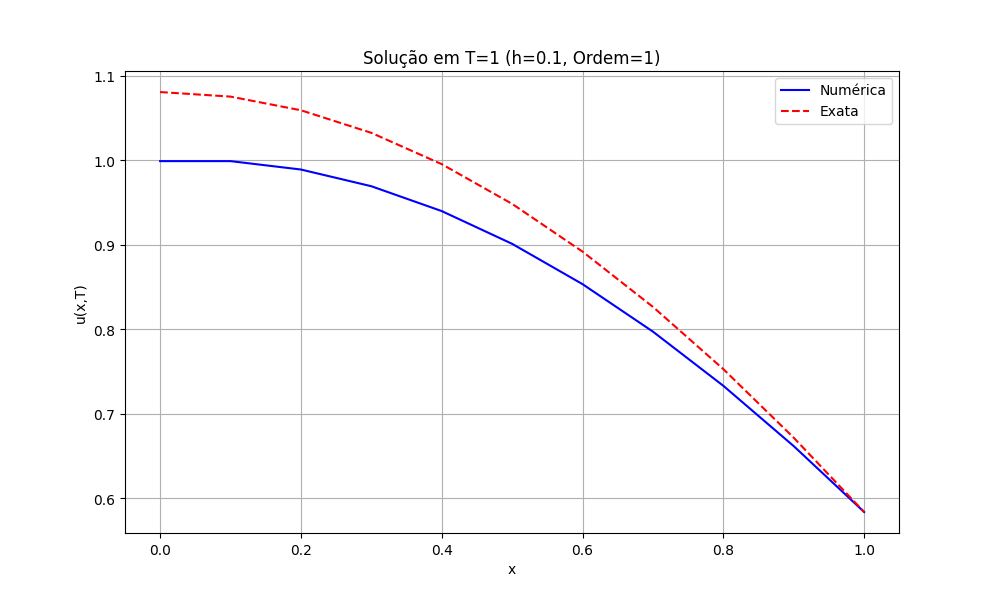
\includegraphics[width=\textwidth]{img/ex0101.png}
		\caption{Solução com $h=0.1$}
		\label{fig:ex1_1}
	\end{subfigure}
	\begin{subfigure}{0.35\textwidth}
		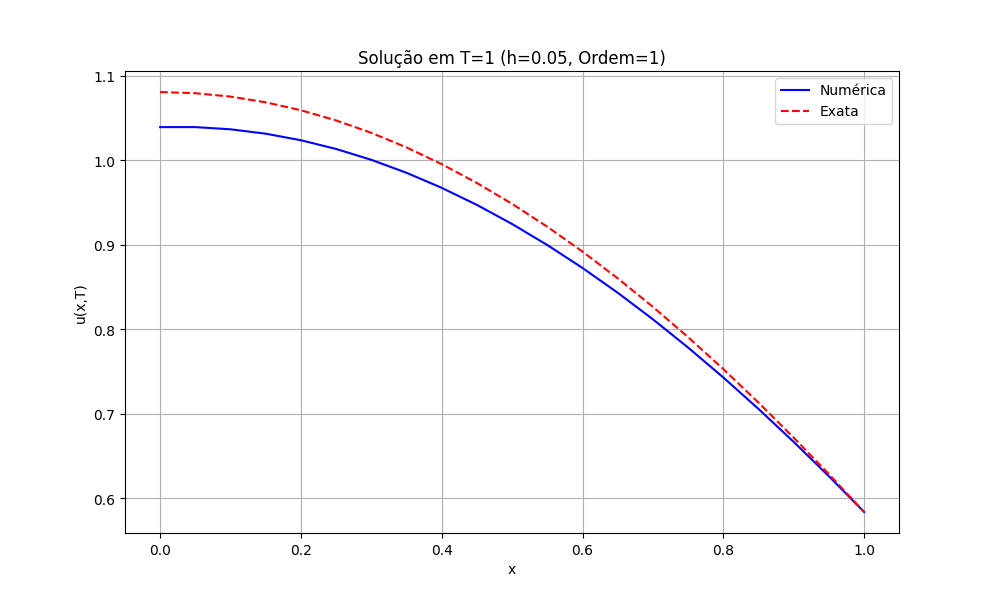
\includegraphics[width=\textwidth]{img/ex0102.png}
		\caption{Solução com $h=0.05$}
		\label{fig:ex1_2}
	\end{subfigure}
	\begin{subfigure}{0.35\textwidth}
		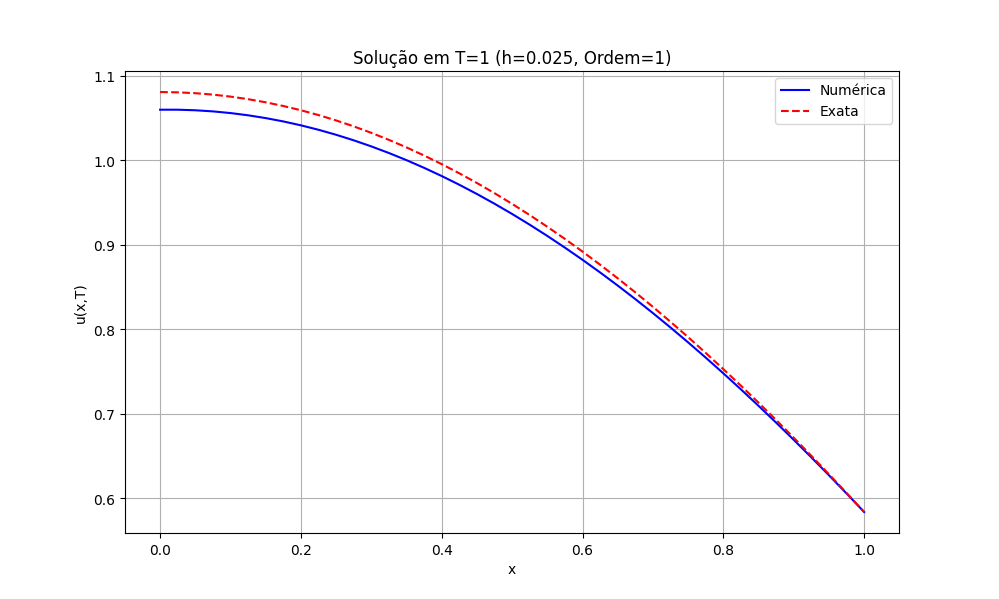
\includegraphics[width=\textwidth]{img/ex0103.png}
		\caption{Solução com $h=0.025$}
		\label{fig:ex1_3}
	\end{subfigure}
	\caption{Soluções numéricas com aproximação de primeira ordem}
	\label{fig:ex1_ord1}
\end{figure}

\begin{figure}[H]
	\centering
	\begin{subfigure}{0.35\textwidth}
		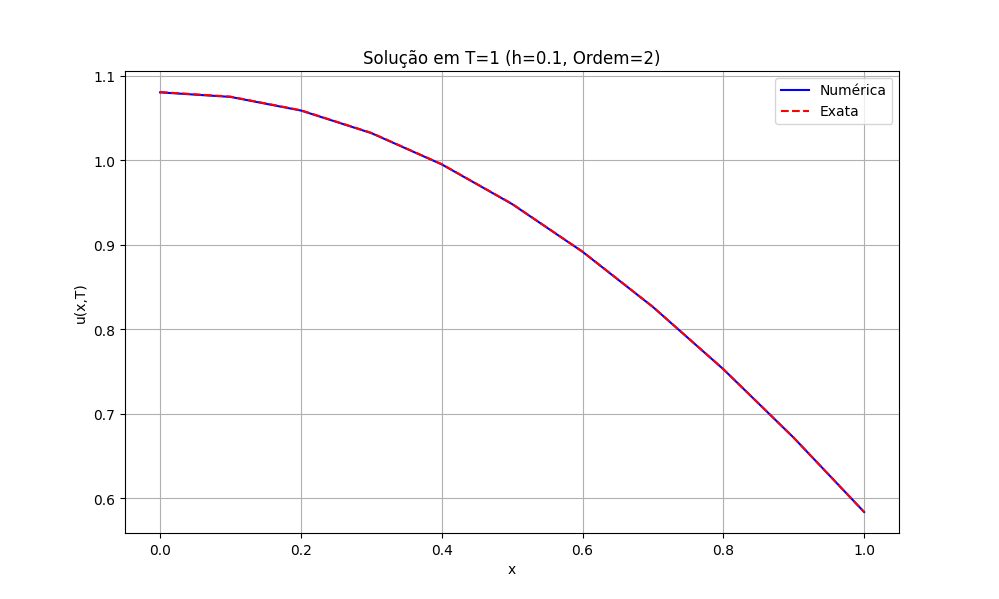
\includegraphics[width=\textwidth]{img/ex0104.png}
		\caption{Solução com $h=0.1$}
		\label{fig:ex1_4}
	\end{subfigure}
	\begin{subfigure}{0.35\textwidth}
		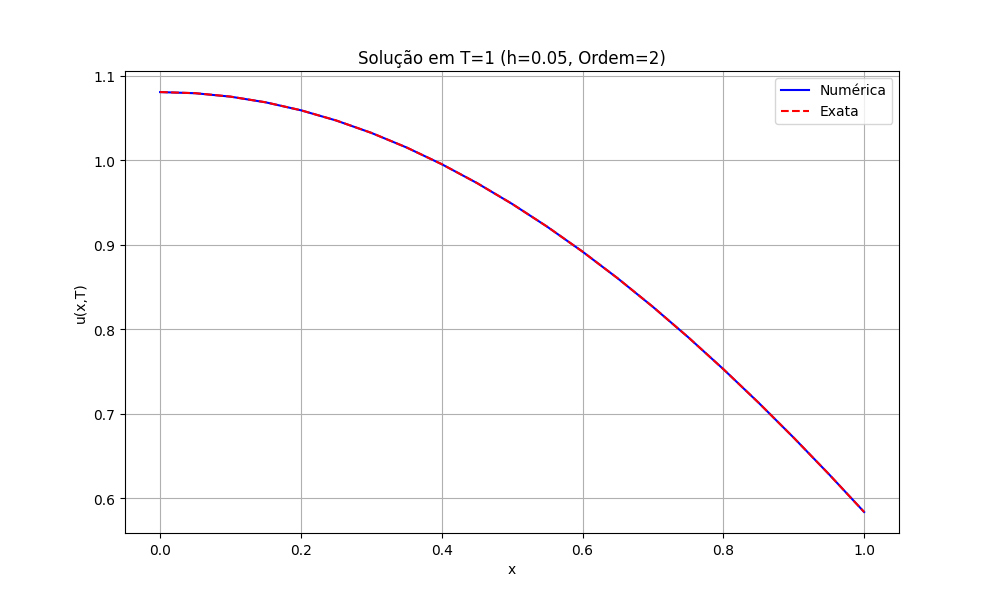
\includegraphics[width=\textwidth]{img/ex0105.png}
		\caption{Solução com $h=0.05$}
		\label{fig:ex1_5}
	\end{subfigure}
	\begin{subfigure}{0.35\textwidth}
		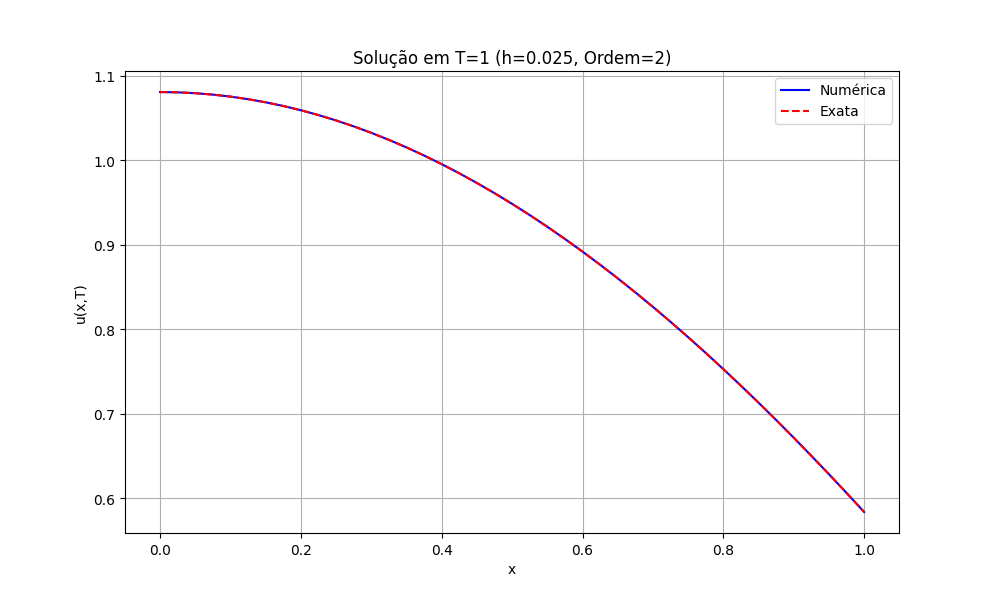
\includegraphics[width=\textwidth]{img/ex0106.png}
		\caption{Solução com $h=0.025$}
		\label{fig:ex1_6}
	\end{subfigure}
	\caption{Soluções numéricas com aproximação de segunda ordem}
	\label{fig:ex1_ord2}
\end{figure}

Note que os gráficos que utilizam aproximação de primeira ordem distanciam-se mais da solução exata ao serem comparados com os gráficos de segunda ordem, ou seja, a partir deste fato, pode-se afirmar que os gráficos de primeira ordem apresentam um erro maior do que os gráficos de segunda ordem. Além disso, à medida que o $h$ diminui, a solução numérica permanece cada vez mais próxima da solução exata, tanto nos gráficos de primeira ordem, tanto nos de segunda.

Por fim, nota-se que tais fatos evidenciados nas figuras, são confirmados pela tabela de cálculo do erro apresentada abaixo:

\begin{table}[H]
	\centering
	\caption{Erro máximo para diferentes valores de $h$ e ordens da condição de Neumann}
	\label{tab:erro_neumann}
	\renewcommand{\arraystretch}{1.25}
	\setlength{\tabcolsep}{12pt}
	\begin{tabular}{|c|c|c|}
		\hline
		\textbf{$h$} & \textbf{Ordem 1} & \textbf{Ordem 2} \\ \hline
		0.1          & 8.171035e-02     & 3.937531e-04     \\ \hline
		0.05         & 4.148152e-02     & 5.096550e-05     \\ \hline
		0.025        & 2.089094e-02     & 6.474309e-06     \\ \hline  
	\end{tabular}
\end{table}

Por fim, analisando a tabela, podemos realizar algumas observações no que diz respeito à ordem de convergência. Para ordem 1, temos que $h$ ao reduzir $h$ pela metade, o erro se reduz aproximadamente pela metade, o que indica uma convergência linear. Já a ordem 2, temos que, ao reduzir $h$ pela metade, o erro reduzir-se em um fator próximo $h^3$, ou seja, uma convergência cúbica.

\subsection{Exemplo 02}

Os gráficos obtidos pelo programa foram:

\begin{figure}[H]
	\centering
	\begin{subfigure}{0.35\textwidth}
		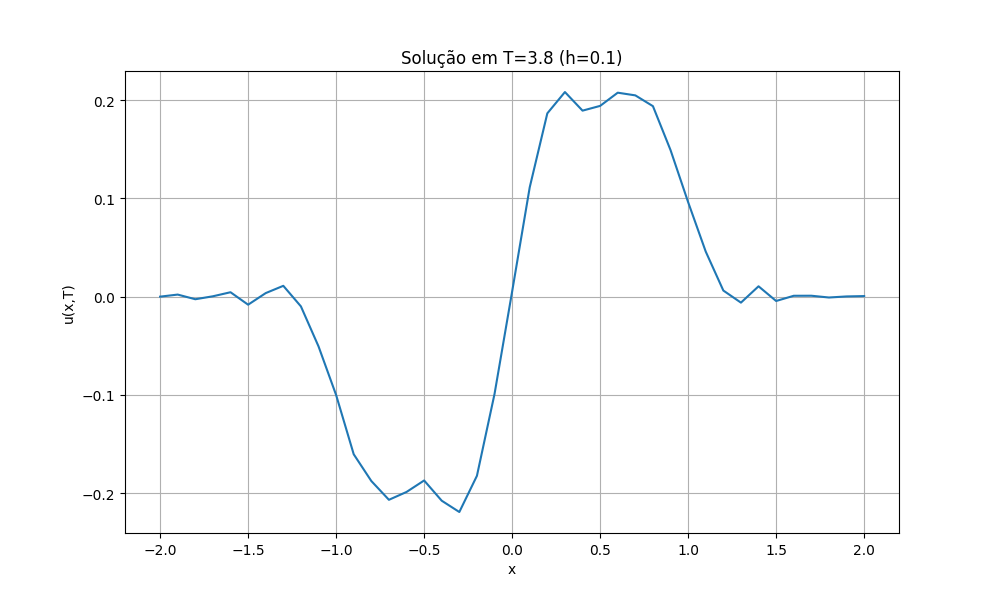
\includegraphics[width=\textwidth]{img/ex0201.png}
		\caption{Solução com $h=0.1$}
		\label{fig:ex2_1}
	\end{subfigure}
	\begin{subfigure}{0.35\textwidth}
		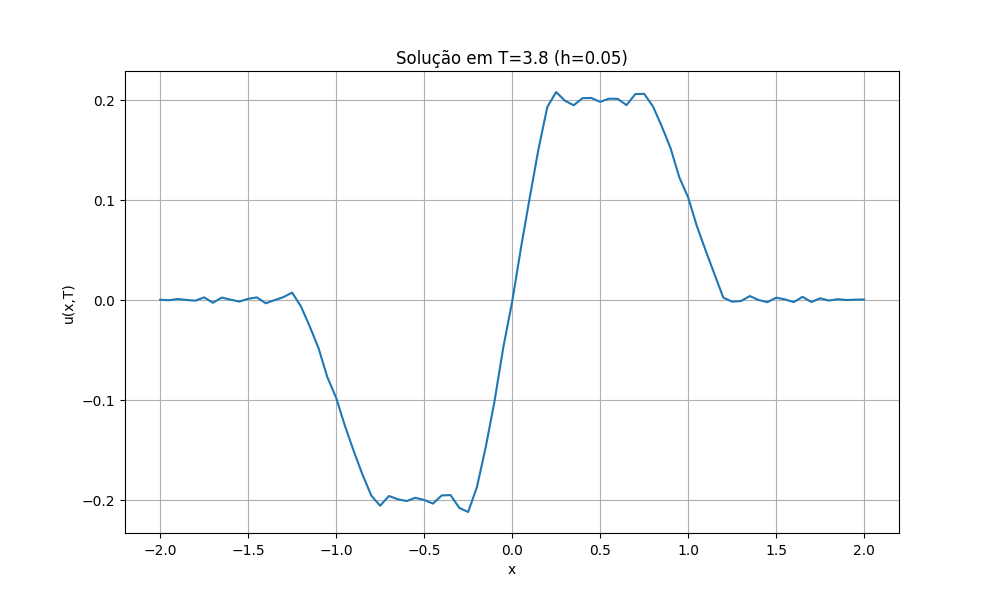
\includegraphics[width=\textwidth]{img/ex0202.png}
		\caption{Solução com $h=0.05$}
		\label{fig:ex2_2}
	\end{subfigure}
	\begin{subfigure}{0.35\textwidth}
		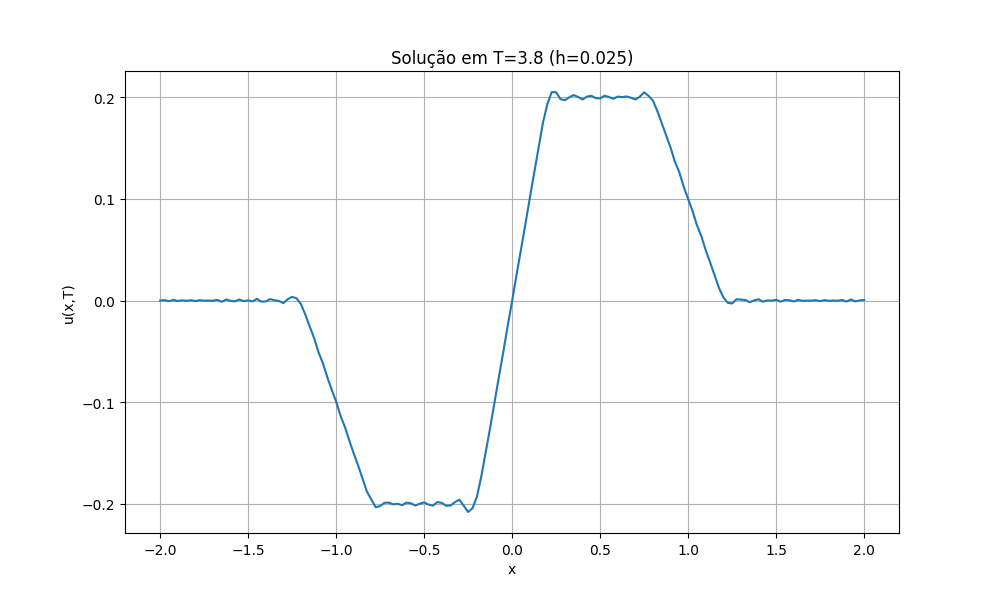
\includegraphics[width=\textwidth]{img/ex0203.png}
		\caption{Solução com $h=0.025$}
		\label{fig:ex2_3}
	\end{subfigure}
	\begin{subfigure}{0.35\textwidth}
		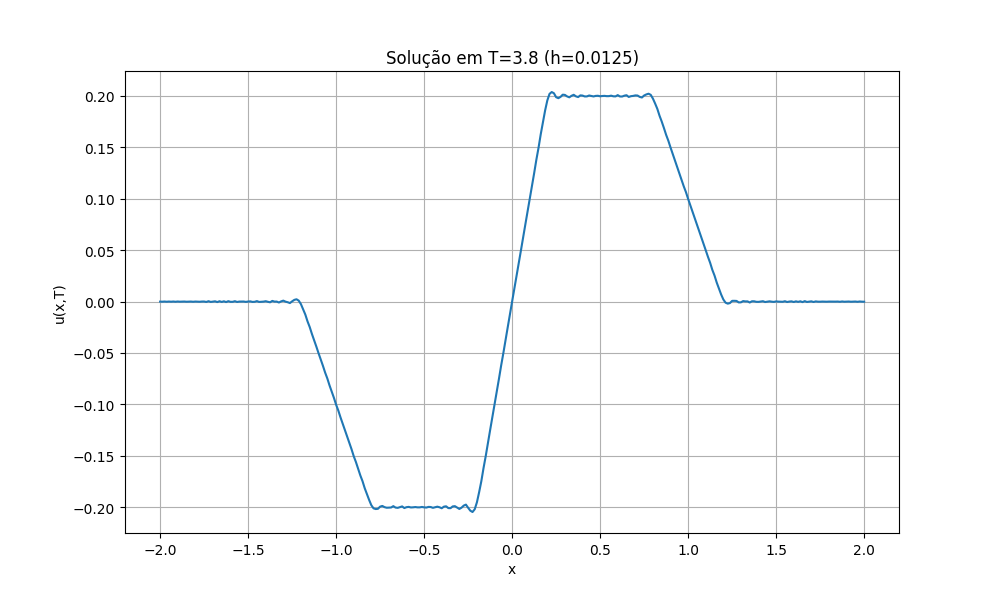
\includegraphics[width=\textwidth]{img/ex0204.png}
		\caption{Solução com $h=0.0125$}
		\label{fig:ex2_4}
	\end{subfigure}
	\caption{Convergência da solução numérica em $T=3.8$ para diferentes valores de $h$}
	\label{fig:ex2_conv}
\end{figure}

Analisando os gráficos, observa-se que o refinamento da malha (redução de $h$) resulta em uma suavização progressiva das oscilações numéricas. Os intervalos $[-2,-1]$, $[-1,0]$, $[0,1]$ e $[1,2]$ apresentam menos perturbações conforme $h$ diminui de $0.1$ para $0.0125$, evidenciando uma melhor aproximação da solução contínua. As transições entre os patamares tornam-se mais suaves, e as regiões planas mostram menos ruído numérico.

Agora, analisando o erro, levando em consideração o que foi posto no enunciado do exemplo: ponto $x=2$ como um ponto de simetria para todo $t$, obtivemos os seguintes resultados para análise do erro:

\begin{table}[H]
	\centering
	\caption{Análise do erro de simetria da solução em T=3.8}
	\label{tab:erro_simetria}
	\renewcommand{\arraystretch}{1.25}
	\setlength{\tabcolsep}{12pt}
	\begin{tabular}{|c|c|}
		\hline
		\textbf{$h$} & \textbf{Erro de simetria} \\ \hline
		0.1000       & 4.160728e-01              \\ \hline
		0.0500       & 4.159548e-01              \\ \hline
		0.0250       & 4.130921e-01              \\ \hline
		0.0125       & 4.072185e-01              \\ \hline
	\end{tabular}
\end{table}

Analisando os dados apresentados na Tabela \ref{tab:erro_simetria}, observa-se que mesmo com sucessivos refinamentos da malha, o erro de simetria permanece praticamente constante na ordem de $10^{-1}$. Esta característica sugere que o refinamento da malha não está sendo eficiente para melhorar a precisão da solução em termos de sua propriedade de simetria, evidenciando uma convergência consideravelmente lenta do método numérico para este aspecto específico do problema.

\subsection{Exemplo 03}

As imagens geradas pelo programa foram:
\begin{figure}[H]
	\centering
	\begin{subfigure}{0.35\textwidth}
		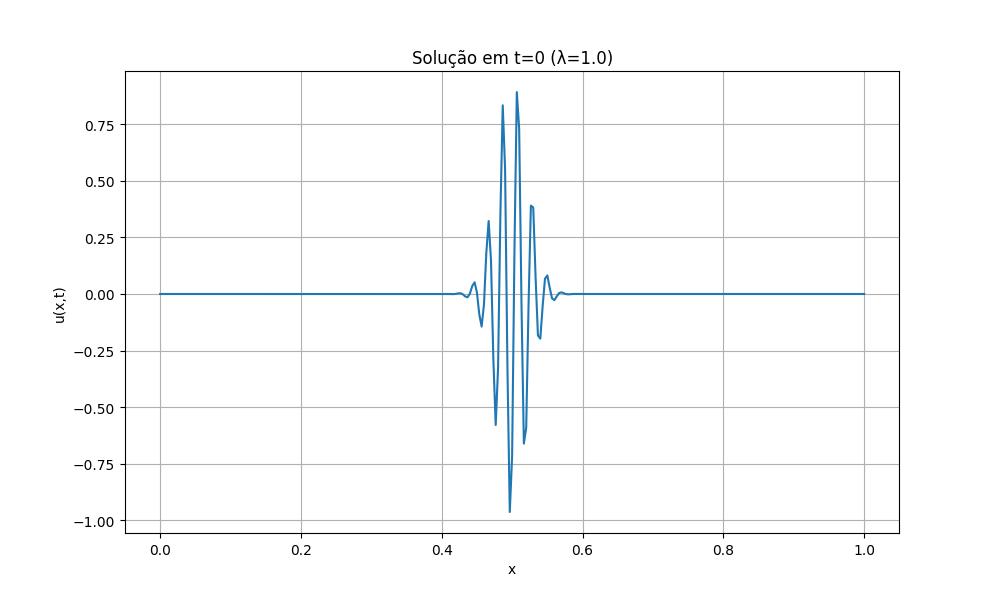
\includegraphics[width=\textwidth]{img/ex0301.png}
		\caption{Pulso inicial em $t=0$}
		\label{fig:ex3_1}
	\end{subfigure}
	\begin{subfigure}{0.35\textwidth}
		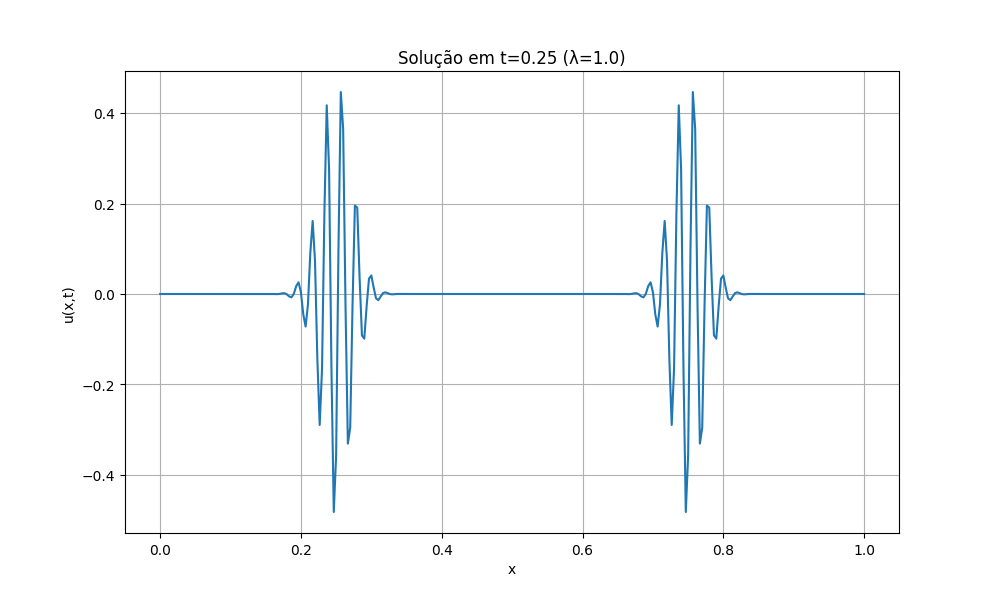
\includegraphics[width=\textwidth]{img/ex0302.png}
		\caption{Separação dos pulsos em $t=0.25$}
		\label{fig:ex3_2}
	\end{subfigure}
	\begin{subfigure}{0.35\textwidth}
		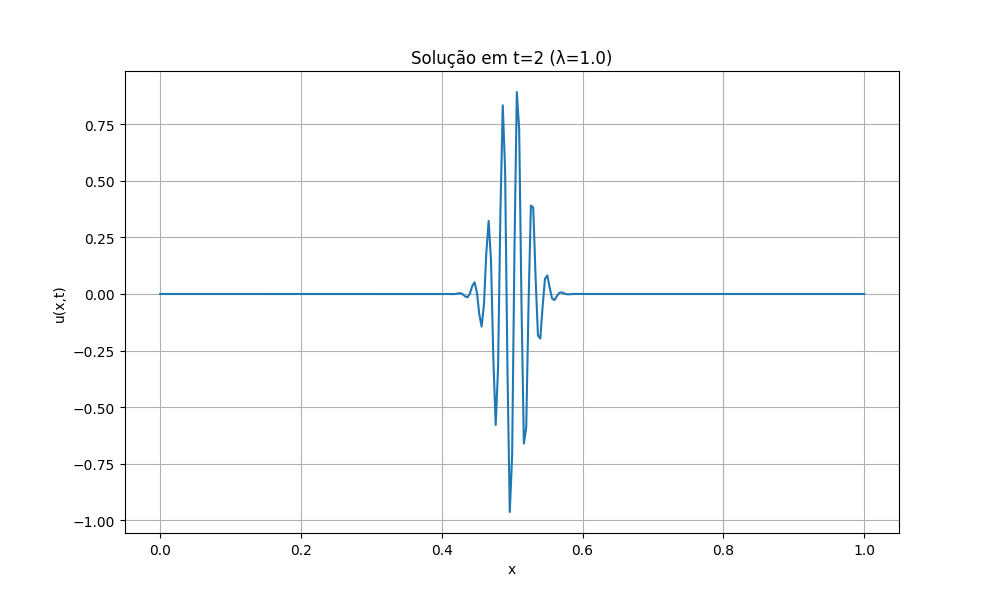
\includegraphics[width=\textwidth]{img/ex0303.png}
		\caption{Solução em $t=2$}
		\label{fig:ex3_3}
	\end{subfigure}
	\begin{subfigure}{0.35\textwidth}
		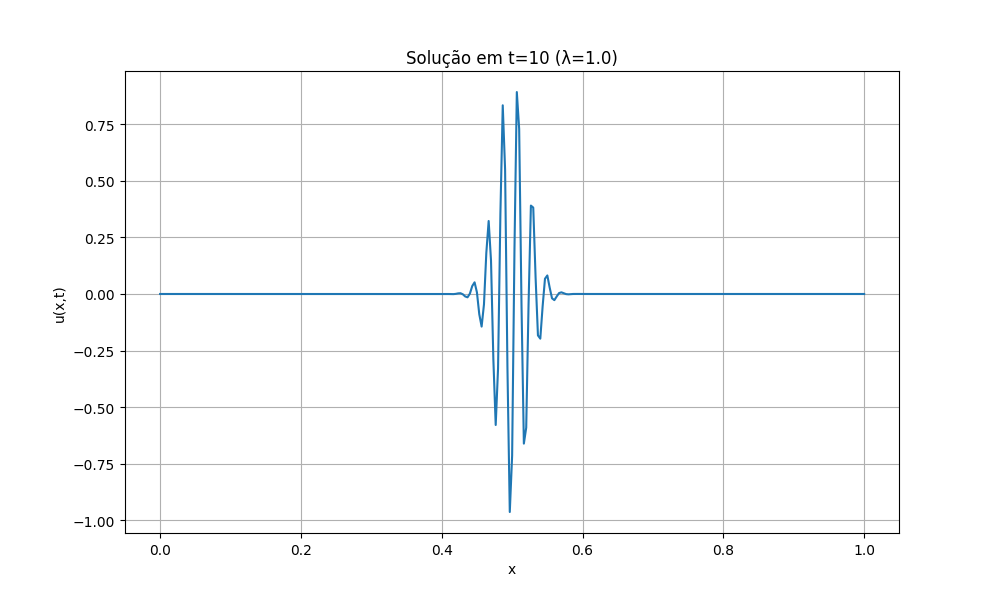
\includegraphics[width=\textwidthUpdate main.py]{img/ex0304.png}
		\caption{Solução em $t=10$}
		\label{fig:ex3_4}
	\end{subfigure}
	\caption{Solução numérica com $\lambda=1.0$ e $h=1/300$}
	\label{fig:ex3_lambda1}
\end{figure}

No primeiro grupo de imagens, quando $\lambda=1$ e $h=300$, temos que as imagens do tempo inicial de $t=0$, $t=2$ e $t=10$ são semelhantes. Enquanto em $t=0.25$ nota-se a presença de duas ondas. Este fato deve-se ao comportamento do objeto estudado

\begin{figure}[H]
	\centering
	\begin{subfigure}{0.35\textwidth}
		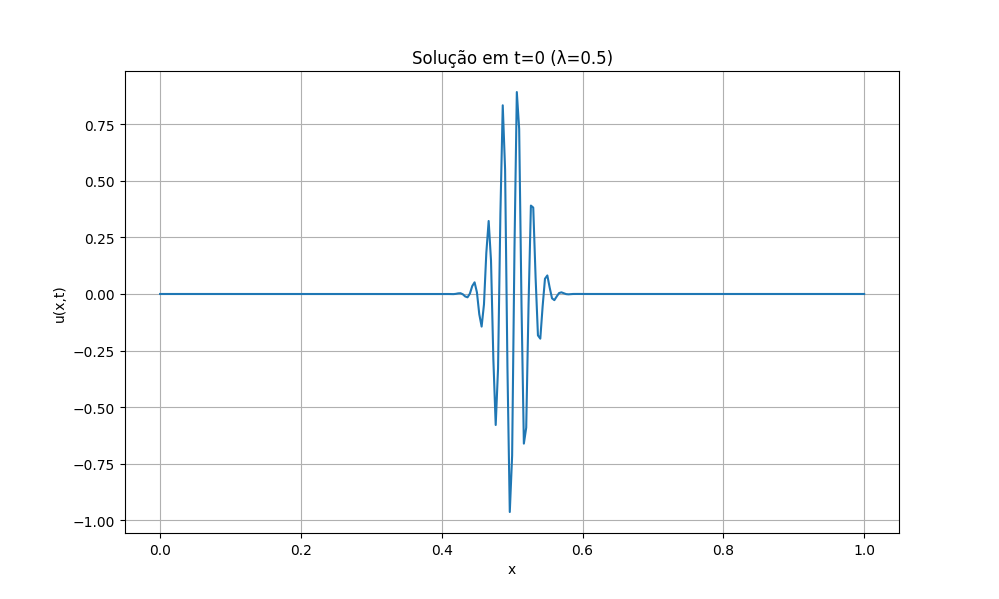
\includegraphics[width=\textwidth]{img/ex0305.png}
		\caption{Pulso inicial em $t=0$}
		\label{fig:ex3_5}
	\end{subfigure}
	\begin{subfigure}{0.35\textwidth}
		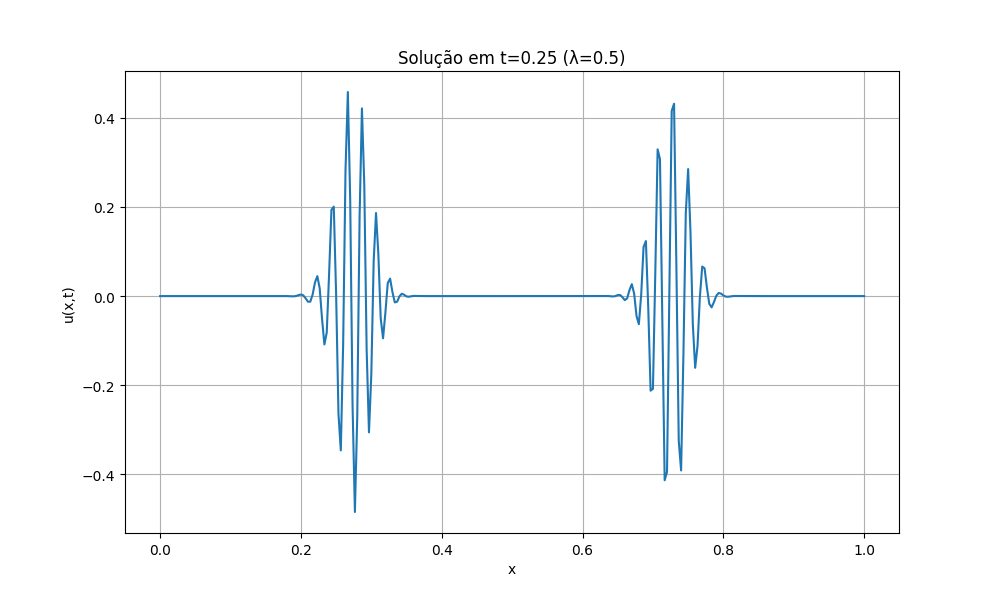
\includegraphics[width=\textwidth]{img/ex0306.png}
		\caption{Separação dos pulsos em $t=0.25$}
		\label{fig:ex3_6}
	\end{subfigure}
	\begin{subfigure}{0.35\textwidth}
		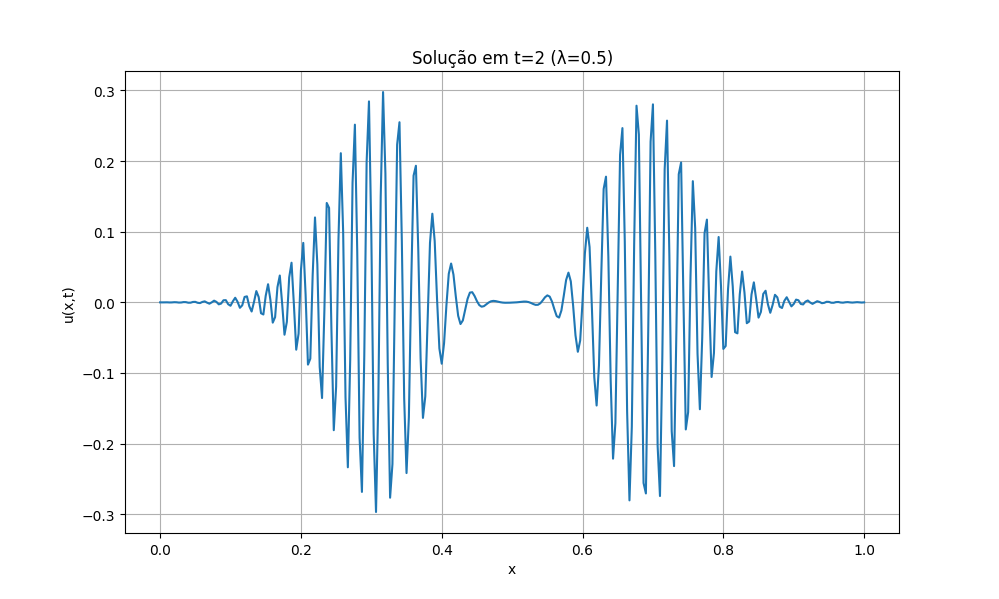
\includegraphics[width=\textwidth]{img/ex0307.png}
		\caption{Solução em $t=2$}
		\label{fig:ex3_7}
	\end{subfigure}
	\begin{subfigure}{0.35\textwidth}
		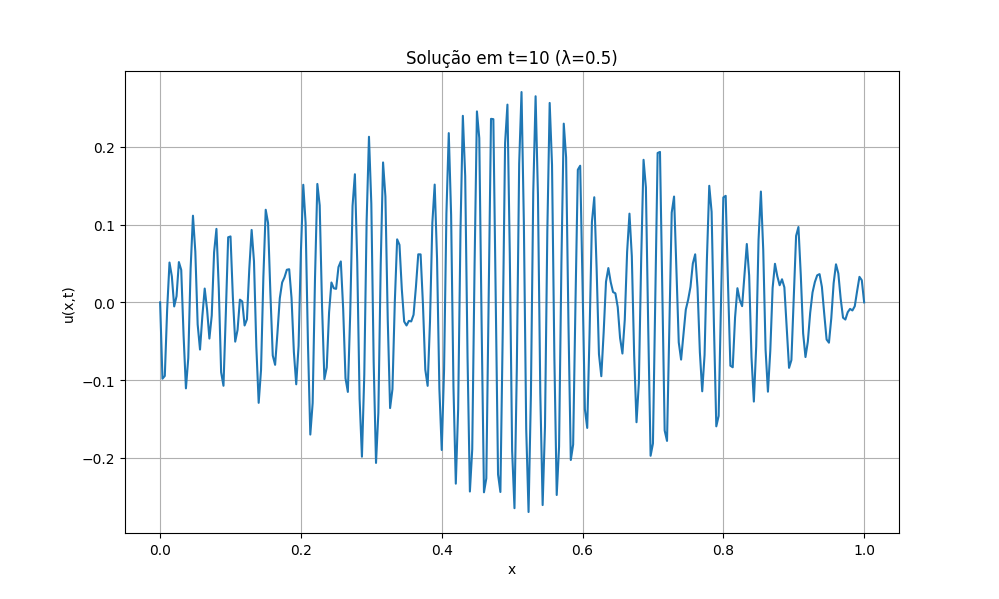
\includegraphics[width=\textwidth]{img/ex0308.png}
		\caption{Solução em $t=10$}
		\label{fig:ex3_8}
	\end{subfigure}
	\caption{Solução numérica com $\lambda=0.5$ e $h=1/300$}
	\label{fig:ex3_lambda05}
\end{figure}

As semelhanças vistas entre os gráficos do mesmo grupo não são vistas no segundo grupo. Em $t=0$ e $t=0.25$, pode-se notar que são semelhantes ao que foi apresentado no primeiro grupo de imagens. Já em $t=2$ e $t=10$, temos que além de serem extremamente diferentes entre si, também são diferentes ao serem comparadas com gráficos do mesmo tempo do grupo anterior. Por fim, é importante destacar o seguinte trecho do enunciado do exemplo 03:
\begin{quote}
	``Quando atingem a fronteira (a primeira vez em $t = 0.5$), eles refletem e então viajam na direção oposta. Nos instantes $t$ iguais a inteiros pares a solução é igual ao seu valor em $t = 0$''. 
\end{quote}

Esse fato pode ser explicado pela periodicidade em relação ao tempo da solução da equação expressa por:
\begin{equation*}
	u(x,2n) = u(x,0), \quad n \in \mathbb{Z}
\end{equation*}

Ela ocorre pelo fato de $c=1$, ou seja, quando a velocidade da onda leva 1 unidade de tempo para percorrer o domínio $L=1$. Além disos, vale destacar que as condições de Dirichlet homogêneas nos extremos causam reflexão com inversão de fase, e após uma ida e volta completa (2 unidades de tempo), a onda retorna à sua configuração inicial, repetindo este ciclo. A respeito à estimação do erro, obtemos a seguinte tabela.
\begin{table}[H]
	\centering
	\caption{Erro em relação à condiçãoUpdate main.py inicial para diferentes valores de $\lambda$}
	\label{tab:erro_lambda}
	\renewcommand{\arraystretch}{1.25}
	\setlength{\tabcolsep}{12pt}
	\begin{tabular}{|c|c|c|}
		\hline
		\textbf{$\lambda$} & \textbf{Erro em t=2} & \textbf{Erro em t=10} \\ \hline
		1.0                & 1.221245e-15         & 3.719247e-15          \\ \hline
		0.5                & 9.634010e-01         & 1.026740e+00          \\ \hline
	\end{tabular}
\end{table}

Para $\lambda=1$, os erros em $t=2$ e $t=10$, apesar de distintos, compartilham a mesma ordem de grandeza ($10^{-15}$), sendo praticamente nulos. Isto confirma a propriedade teórica do esquema ser exato quando $c\lambda=1$. O mesmo não se pode dizer em relação à $\lambda=0.5$: apesar de terem valores relativamente próximos (uma diferença de $6\times10^{-2}$), há acumulação de erros numéricos ao longo do tempo, mesmo com passo temporal menor. 

\section{Conclusão}
Concluí-se que o Método de Diferenças Finitas (MDF) demonstrou-se uma ferramenta eficaz para a resolução numérica de equações de onda unidimensionais da forma apresentada em \eqref{eq:equacao-da-onda}, sujeitas às condições iniciais expostas em \eqref{eq:condicao-inicial-onda}.

No presente trabalho, foram desenvolvidos três exemplos distintos que, embora compartilhem a natureza de fenômenos ondulatórios unidimensionais, apresentaram características únicas. Cada exemplo permitiu explorar diferentes aspectos da aproximação numérica: o primeiro possibilitou uma análise quantitativa e visual da convergência através da comparação direta entre soluções exata e numérica; o segundo explorou propriedades de simetria em torno de $x=2$ e sua preservação numérica; e o terceiro demonstrou a capacidade do método em capturar fenômenos físicos como a propagação, reflexão e periodicidade de pulsos ao longo do tempo.

Um aspecto crucial evidenciado foi a sensibilidade do método aos parâmetros numéricos. Em particular, a escolha de $\lambda = \tau/h$ mostrou-se determinante para a precisão e estabilidade das soluções. No primeiro exemplo, observamos como diferentes ordens de aproximação para a condição de Neumann afetam a convergência. No segundo, vimos que mesmo com refinamento da malha, certas propriedades geométricas podem ser difíceis de preservar numericamente. Já no terceiro exemplo, a comparação entre $\lambda = 1$ e $\lambda = 0.5$ demonstrou como a escolha dos parâmetros pode afetar a precisão da solução em tempos longos, com o caso $\lambda = 1$ produzindo resultados mais precisos.

\section{Referências}
\nocite{*}
\printbibliography[heading=none]

\end{document}